\documentclass[main.tex]{subfiles}
\begin{document}
	
	\chapter{Manipulation}
		\chapterauthor{Marc Stelter, Jan Neuman \& Fabian Weihe}
	
	\subsection{General}
	Manipulation has four Actionservers.\\
	The "move\_gripper\_action\_server" moves the gripper to the given position.\\
	The "take\_pose\_action\_server" moves the robot into perceiving position.\\
	The "grasps\_object\_server" receives the size and position of an object and grasps it.\\
	The "place\_server" places the attached object at the given pose.\\
	Further Manipulation has a "suturo\_manipulation\_launch" package, which launches the Actionservers, rviz and giskard and a "object\_state\_listener" package.
	
	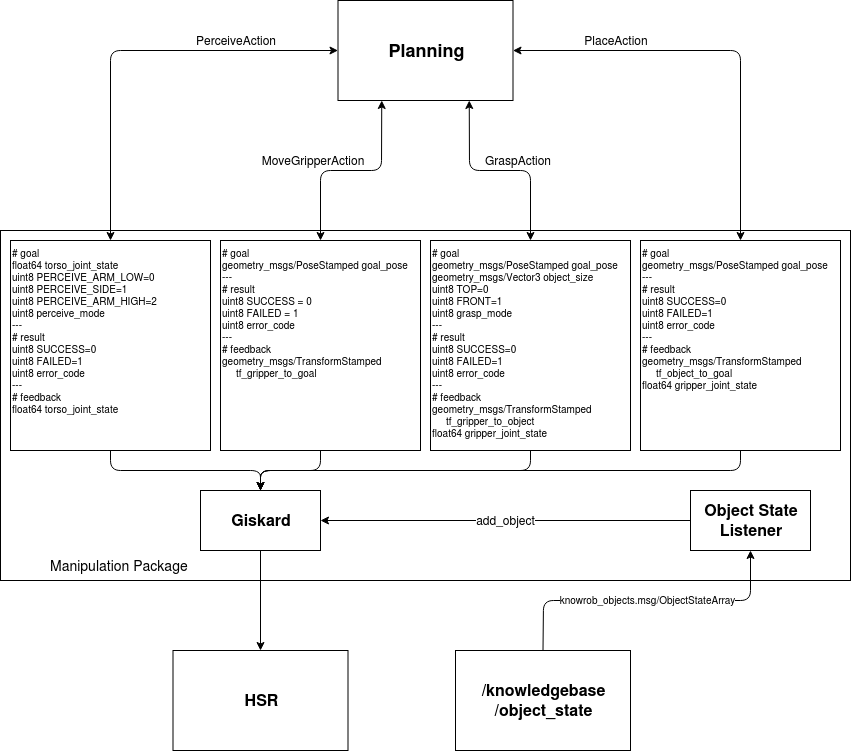
\includegraphics[scale=0.5]{pictures/Manipulation.png}
	
	\subsection{Move Gripper}
	The received pose is simply forwarded as a cartesian goal to giskard, which in turn will take care of the collision avoidance and movement. Giskards error\_code gets returned to the client.
	\vspace{1cm}
	
	\subsection{Take perceiving Pose}
	The Take Pose Action Server gets a Vector3 gaze\_point, an int perceive\_mode and all joint values as float from the client. The gaze\_point is a coordinate in map that tells the server to which point the camera should look. The perceive\_mode describes the mode that the server should use to put the robot in a good perceiving position. The purpose of the joint values is that planning can move the robot into any given pose in "FREE" mode. In modes "LOOK\_HIGH", "LOOK\_LOW" and "NEUTRAL" the server moves all joints into a predefined pose that is chosen in "perceive\_mode". In the "GAZE" mode the server moves all joints except head joints and "arm\_lift\_joint" into a position where the arm is not blocking the cameras view. Then the correct height for "arm\_lift\_joint" is calculated and the head is panned and tilted in the right direction to perceive the given object coordinates. When the action is finished either SUCCESS or FAILED are returned to the client.

	\vspace{1cm}
	
	\subsection{Grasps Object}
	The server receives a PoseStamped ("goal\_pose"), a Vector3("object\_size") and a "grasp\_mode". In the first step the script opens the gripper to the maximum. After that the arm is moved to the object. The "grasp\_mode" determines if the object should be grasped from the front or the top or a free given orientation. When the arm has moved to the given position "goal\_pose", the script closes the gripper. At the end the grasped object given by "object\_frame\_id" is added in giskard and attached to the robot. Then the server transforms to a position, where it can comfortably move with an object in the gripper.\\
	Finally it checks if the object is in the gripper and returns whether the action has failed or succeeded.
	
	\vspace{1cm}
	
	\subsection{Place Object}
	The object "object\_frame\_id" that was attached by the grasp server is moved to the goal position "goal\_pose". The "place\_mode" defines the orientation in which the object should be placed. In order to release the gripper the HSR Python interface is used directly. Finally the object is detached and the "error\_code" is returned.
	
	\vspace{1cm}
	
	\subsection{Object State Listener}
	The object state listener is responsible for taking an "object\_state\_array" from knowledge and adding this given object to giskard for the action servers to use.
	
	\vspace{1cm}
	
	\subsection{Launch}
	The "Launch" package contains a Launchfile to launch the Actionservers with their dependencies. The file includes five arguments.\\
	The first one is a boolean called "sim". On false giskard is launched to work on the real robot. Otherwise on true giskard is launched to work in a simulation. Additional to that the iai\_hsr\_sim is launched for the simulation.\\
	The other four arguments are booleans, too. Which defines whether an actionserver should start. 
\end{document}
